\centerline{\bf \Huge Домашнее задание}
\centerline{\bf \Huge Осевая симметрия}

\begin{flushright}
        \scriptsize{Последовательность - враг предпринимательства,\\ точно так же, как симметрия - враг искусства.\\Джон Бернард Шоу.}
\end{flushright}

\problem{1}
а) На листе прозрачной бумаги нарисован угол. Как без всяких инструментов построить биссектрису этого угла? После этого покажите, как построить центр вписанной
окружности для треугольника, нарисованного на той же прозрачной бумаге.

б) На листе прозрачной бумаги нарисован отрезок. Как без всяких инструментов построить серединный перпендикуляр к этому отрезку? После этого покажите, как построить центр описанной окружности для треугольника, нарисованного на той же
прозрачной бумаге.

\problem{2}
Из квадратного листа бумаги сложили треугольник (см. рисунки). Найдите отмеченный угол.

\begin{center}
    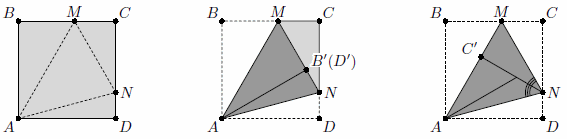
\includegraphics[width=0.75\textwidth]{ЭлМШ 2024-2025/II блок/Геометрия/image.png}
\end{center}

\problem{3}
Барон Мюнхаузен утверждает, что пустил шар от борта бильярда, имеющего форму правильного треугольника, так, что тот, отражаясь от бортов, прошёл через некоторую точку три раза в трёх различных направлениях и вернулся в исходную точку. Могут ли слова барона быть правдой? (Отражение шара от борта происходит по закону "угол падения равен углу отражения".)

\problem{4}
На биссектрисе внешнего угла $C$ треугольника $ABC$ взята точка $M$, отличная от $C$. Докажите, что  $MA + MB > CA + CB.$

\problem{5}
В равнобедренном треугольнике $ABC (AB = AC)$ биссектриса $BL$ пересекается с биссектрисой угла $A$ в точке $I$. Точка X на стороне AB выбрана так, что $BX = BC$. Прямая $XI$ пересекает основание $BC$ в точке $Y$. Докажите, что $BY = CL.$